\chapter{Problemanalyse}
\textit{I dette kapitel analyses problemstillinger, som opstår i forbindelse med lægemiddelskift. Disse problemstillinger vil sammenfattes i en opsummering og afsluttes med en problemformulering, der fremadrettet danner  grundlaget for rapporten.}

\section{Lægemiddelskift}
Lægemiddelskift forekommer når en ny lægemiddelvirksomhed vinder leverancen af nyt lægemiddel som standardbehandling, hvormed der er indgås et kontraktskift~\citep{Amgros2015}. 

Forinden et kontraktskift kan forekomme analyseres og vurderes lægemidlet i samarbejde med Medicinrådet og Amgros~\citep{DanskeRegioner2016}, som beskrevet i Appendiks \ref{cha:AppA}. Efter analyseringen og vurdering sendes lægemidlerne i udbud via Amgros med henblik på at indkøbe lægemidler af høj kvalitet til bedst mulige pris~\citep{Sygehusapoteket2017}.

Størstedelen af lægemidler i ATC-grupper sendes i udbud en gang årligt fra start september til midt november, hvor udbud på ATC-grupper som indgår i Medicinrådets behandlingsvejledninger sker løbende hen over året~\citep{Sygehusapoteket2017}, som beskrevet i Appendiks \ref{cha:AppD}.
Forinden udbuddet defineres antallet af vindere samt, hvorvidt udbuddet skal vurderes på baggrund af laveste pris eller være mest økonomisk fordelagtigt~\citep{Amgros2018a}, som beskrevet i Appendiks \ref{cha:AppB}.

På baggrund af de foregående analyser og vurderinger fastsættes et prisniveau der anvendes som beslutningsgrundlag for Medicinrådet om, hvorvidt lægemidlet skal anvendes som standardbehandling~\citep{DanskeRegioner2016}. Hvis lægemidlet er den eneste standardbehandling inden for terapiområdet kan denne implementeres direkte på hospitalsafdelingen. I tilfælde af flere lægemidler inden for samme terapiområde, skal lægemidlernes ligeværdighed vurderes af Medicinrådet, som beskrevet i Appendiks \ref{cha:AppA}, med henblik på at udarbejde behandlingsvejledninger og rekommandationer for lægemidlerne. Disse videresendes til de danske hospitaler, som står for implementeringen.~\citep{DanskeRegioner2016}

\section{Substitution of lægemidler}
Kontraktskift medfører enten analog eller generisk substitution af lægemidler, hvor et lægemiddel udskiftes til et andet lægemiddel~\citep{DanskSelskabforPatientsikkerhed2009}.
Generisk substitution, er ifølge The World Health Organisation (WHO), defineret som dispensering af et produkt, der er generisk ækvivalent med det foreskrevne produkt med samme aktive ingredienser i samme doseringsform og identisk i styrke, koncentration og administrationsvej~\citep{Kairi2017}. Generisk substitution kan f.eks. være skift fra Paracetamol til Crocin eller ændring i mærke som Pamol til Pinex~\citep{Kairi2017} 

Analog substitution er defineret af WHO som substitutionen af et lægemiddel med et andet, der afviger i sammensætningen, men anses for at have lignende bivirkninger og terapeutiske egenskaber~\citep{Kairi2017}. Med andre ord vil dette sige at alle substitutioner som ikke er generiske er analoge. De fleste analog substituerede lægemidler afviger fra det foreskrevne lægemiddel på baggrund af optagelsen af lægemidlet f.eks. ændring fra et lægemiddel med hurtigt frigivelse til et med langsom, eller at lægemidlet anvender et alternativ molekyle fra samme farmakologiske klasse~\fxnote{losartan i stedet for telmisartan}. I sjældnere tilfælde anvendes lægemidler hvor det alternative molekyle er for en anden farmakologisk klasse~\fxnote{telmisartan i stedet for ramipril}.~\citep{Kairi2017}

\section{Ulemper ved substitution af lægemidler}
Ulemperne ved generisk substitution er at der gives et andet lægemiddel end ordineret af lægen~\citep{Kairi2017}. Selvom lægemidlet indeholder somme aktive stof kan producenten af lægemidlet anvende forskellige hjælpestoffer, som på trods af kliniske forsøg, kan vise signifikante forskelle for nogle patienter i forhold til interaktion af lægemidler og optagelse af lægemidlet. En anden ulempe er at den generisk substitution kan medfører at erstatningens lægemidlet har et anderledes udseende som f.eks. form, størrelse og farve på dispenseringsformen, hvilket kan medvirke til at patienten mistænker en fejl i ordinationen og derved udelader at tage medicinen.~\citep{Kairi2017}

Foruden de ulemper som er beskrevet omkring generisk substitution er ulemperne ved analog substitution at nogle lægemidler inden for samme farmakologiske klasse afviger væsentligt fra deres biologiske virkning~\citep{Kairi2017}. Det er endnu ikke påvist hvilken betydning dette har for den terapeutiske virkning. Patientens holdning, accept og forståelse har en påvirkning på analog substitution. Hvis patienten fejlinformeret eller ikke har fået den rette information omkring analog substitution kan dette indbærer et indtryk af utilstrækkelig eller uhensigtsmæssig behandling~\citep{Kairi2017}.
 
%Der findes to typer af substitution herunder analog og generisk. Analog substitution omhandler lægemidler der indeholder forskelligt aktivt lægemiddelstof, har nogenlunde ens effekt og bivirkninger. Disse kræver ændring i ordination og skal derfor ordineres af en læge. Generisk substitution omhandler lægemidler som indeholder det samme virksomme lægemiddelstof og fungerer derfor som hinandens synonyme. Dette skift kræver ikke en ændring i ordination og kan derfor varetages af en sygeplejerske.~\citep{DanskSelskabforPatientsikkerhed2009}

\section{Implementering af substituerede lægemidler}
Et simpelt lægemiddelskift er vurderet til at påvirke hospitalsafdelingen i lav grad og varetages ofte af logistik afdelingen~\citep{Laegemiddelinformaion2017, Sygehusapoteket2017a}. Disse skift sker dagligt og kan forekomme i forbindelse med ændring af generisk navn eller ved ændring af lægemidlets mærke~\citep{Sygehusapoteket2017a, Kairi2017}. Hvorimod et kompleks lægemiddelskift påvirker klinikken i mellem til høj grad og kræver ofte involvering af flere interessenter som f.eks. medicinansvarlig, overlæger, kontaktsygeplejersker eller medicinservicefarmakonomer til at undersøge lægemidlets anvendelighed for det pågældende hospitalsafsnit. 
De komplekse skift sker ved lægemidler, hvor flere faktorer som f.eks. styrke og disponeringsform afviger fra den nuværende behandling.~\citep{Laegemiddelinformaion2017,Sygehusapoteket2017a}

\section{Patientsikkerhedsmæssige konsekvenser ved substituion} \label{sec:ProblemLaeg}
Substitution af lægemidler kan medføre patientsikkerhedsmæssige konsekvenser~\citep{DanskSelskabforPatientsikkerhed2009}. 
Et norsk studie har undersøgt konsekvenserne ved generisk substitution~\citep{Hakonsen2010}. Interview med 100 sygeplejersker påviste at der opstod fejlmedicinering ved generiske lægemidler~\citep{Hakonsen2010}. Ud af disse følte 92~\% af sygeplejerskerne at generiske lægemidler var tidskrævende og 91~\% at risikoen for fejl øges ved dispensering af disse, hvoraf 42~\% oplevede fejl som følge af generisk substitution~\citep{Hakonsen2010}.
Medicineringsfejl ved generisk substitution fremgår af Figur \ref{fig:GeneriskSubstitution}.

\begin{figure}[H]\centering	\includegraphics[width=1\textwidth]{billeder/GenSub.png} 
	\caption{Medicineringsfejl ved generisk substitution rapporteret (n=100)~\citep{Hakonsen2010}.}
	\label{fig:GeneriskSubstitution}  
\end{figure}

Det fremgår af Figur \ref{fig:GeneriskSubstitution} at størstedelen af fejlmedicinering ved generisk substitution skyldes forkert lægemiddel, hvoraf en mindre del skyldes forkert formulering og i sjældnere tilfælde forkert dosis, administrationsvej og udeladelse af dosis. Forkert lægemiddel forstås som at et andet lægemiddel end det oprindelige er dispenseret. Formulering beskriver lægemidlet fysiske form som f.eks. tabelletform, dosis beskriver mængden af lægemidlet og administrationsvej beskriver hvordan indgiften af et lægemiddel tages f.eks. via munden.

Det norske studie undersøgte ligeledes årsagerne til medicineringsfejl, hvilket er rapporteret af 42 sygeplejersker~\citep{Hakonsen2010} og fremgår af Figur \ref{fig:GeneriskSubstitution1}.

\begin{figure}[H]\centering	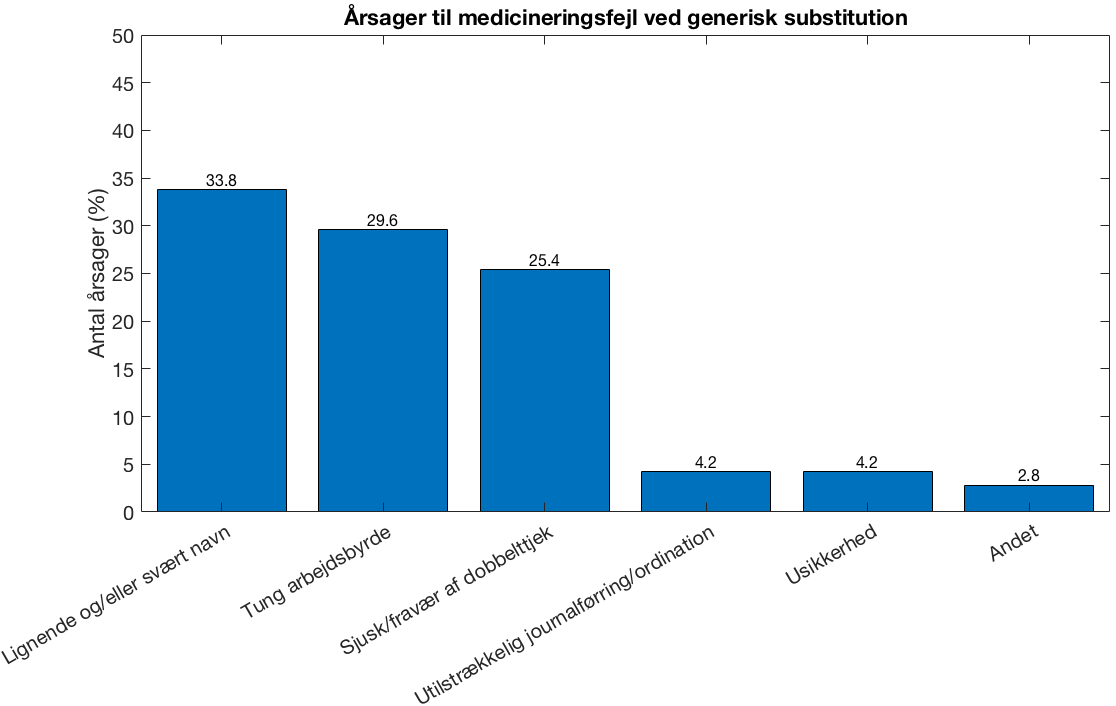
\includegraphics[width=1\textwidth]{billeder/GenSub1.png} 
	\caption{Årsager til medicineringsfejl ved generisk substitution (n=42)~\citep{Hakonsen2010}.}	\label{fig:GeneriskSubstitution1}  
\end{figure}

Af Figur \ref{fig:GeneriskSubstitution1} fremgår det at størstedelen af årsagerne til medicineringsfejl ved generisk substitution skyldes lignende og/eller vanskeligt lægemiddelnavn, kraftig arbejdsbyrde og sløvhed eller fravær af dobbelttjek. En mindre del skyldes utilstrækkeligt journalførring og/eller ordination, usikkerhed eller andet. 

I flere lande, inklusiv Danmark, opstår forkert lægemiddel ofte i forbindelse med forvirring ved forveksling af navn eller emballage~\citep{DanskSelskabforPatientsikkerhed2009}, hvilket afspejles i det norske studie. Forveksling af lægemiddelnavne har i sjældnere tilfælde haft konsekvenser som har medført forlænget indlæggelse, forværret sygdom eller dødsfald.~\citep{DanskSelskabforPatientsikkerhed2009}

Forveksling af navn kan for eksempel forekomme ved panodil, som er et smertestillende lægemiddel, og plendil, som anvendes til behandling af forhøjet blodtryk~\citep{DanskSelskabforPatientsikkerhed2009}. Derudover kan forskellige suffiks eller præfiks skabe forvirring og give anledning til fejl dispensering såsom Efexor kontra Efexor Depot og Levemir penfill kontra Levemir flexpen.~\citep{DanskSelskabforPatientsikkerhed2009} Udover selve lægemidlets navn kan lægemidler som har lignede navne, så kaldte look-a-like, prædisponeres til medicineringsfejl som kan have patientsikkerhedsmæssige konsekvenser~\citep{Wittich2014}. Eksempler på look-a-like lægemidler er  dopamin, som anvendes  og dobutamin, daunorubicin og doxorubicin, vincristin og vinblastin samt prednison og prednisolon~\citep{Wittich2014}. Brugen af forkortelser i ordinationen eller kommunikation medfører ligeledes til øget risiko for medicineringsfejl~\citep{Wittich2014}. Et eksempel på dette kan være  forveksling mellem enheder som international enheder (IE) og intravenøs (IV)~\citep{Wittich2014}. 

Nogle af sygeplejerskerne i det norske studie mente at forvirringen over at finde den korrekte substitution kunne lede til at dosering og formulation var skyld i medicineringsfejl~\citep{Hakonsen2010}. Kognitive forstyrrelser, som fejl ved bekræftelse eller mangel på situationsfornemmelse, kan bidrage til medicineringsfejl. Et eksempel på dette kan være forvirring over lægemidlets placering, hvis den oprindelige placering er ændret og et andet lægemiddel står på denne plads. Det samme paradoks kan forekomme hvis lægemidlets leverandør ændres hyppigt, hvormed det nuværende lægemidlet skal substitueres til et andet~\citep{Wittich2014}

I takt med at hospitalets medicin opgørelse gennemgår ændringer jævnligt og antallet af generiske  substitutioner stiger medvirker dette til at arbejdsbyrden er steget~\citep{Hakonsen2010}. Til trods for at sygeplejerskernes arbejde er blevet mere kompleks og krævende har de kun modtaget en begrænset oplæring inden for området.~\citep{Hakonsen2010} I forhold til sjusk og fravær af dobbelttjek blev det i det norske studie rapporteret af 27~\% sygeplejersker at det var kutyme at en anden sygeplejerske dobbelttjekkede medicinen før den blev givet til patienten~\citep{Hakonsen2010}. Yderligere angav 48~\% at dobbelttjekket kun skete i de tilfælde hvor de var usikre.~\citep{Hakonsen2010} 

Medicinering var den hyppigste årsag til rapportering af utilsigtede hændelser i år 2013~\citep{Patientombuddet2013}. Antallet af rapporteringer i Region Nordjylland er steget med over 36~\% fra år 2012 til 2014~\citep{Jensen2014}. Ud af 824 rapporterede utilsigtede hændelser i år 2014 omhandlede 97\% medicinering, 86\% administration af medicin og 41\% disponering~\citep{Jensen2014}, hvor mere end en rapporteret  utilsigtede hændelser kan skyldes en eller flere grunde. 
Håndteringen af medicin er kompleks, da det er en mangeartet operation som involverer flere personer og mange led, herunder ordination, transskribering, dispensering og administration. I alle led i processen er der påvist fejl~\citep{Barker2002,Sundhedsstyrelsen2005, Lisby2005, Tully2009}, hvor størstedelen af fejl forekommer i forbindelse med ordination og administration og en mindre andel af fejl ved transskribering og dispensering~\citep{Agrawal2009, Anderson2002} 
En fælles årsag til rapporterede utilsigtede hændelser i disse studier var forkert dosis, forkert lægemiddel og udeladelse af henholdsvis ordination, dispensering og administration~\citep{Barker2002,Sundhedsstyrelsen2005,Lisby2005, Tully2009}.
Størstedelen af medicineringsfejl ved ordination inkluderer brug af forkert lægemiddel, doseringsform, styrkeberegning, manglende kontrol af allergier og manglende evne til at justere doseringen hos patienter med nedsat nyre- eller leverfunktion.~\citep{Agrawal2009}.


%\section{Forebyggelse af problemstillinger ved lægemiddelskift}
%Den europæiske lægemiddelstyrelse har udviklet vejledninger med henblik på at forebygge problemer opstået ved forveksling af lægemidler og derved reducere antallet af medicineringsfejl~\citep{DanskSelskabforPatientsikkerhed2009}. Disse vejledninger er ikke indført i Danmark, men der har været fokus på problemer med emballage forvekslinger, hvormed lovgivningen i Danmark er at pakninger ikke må kunne forveksles.   

%Udover vejledninger har internationale studier påvist at stregkode teknologi reducerer antallet af fejl i medicineringsprocessen~\citep{Poon2006, Levtzion-korach2010} Stregkode teknologi kan anvendes til at sikre at den rette medicin modtages af den rette patient~\citep{Amgros2013}.  
%Amgros har siden år 2010 stillet krav til stregkode på yderste og inderste emballage på lægemidler~\citep{Amgros2013}. Foruden at undgå alvorlige medicinrelaterede fejl kan stregkoder medfører en mere enkel og sikker registrering af lægemidler i patienternes medicinjournal og effektiv tilbagekaldelse af medicin via it-systemer~\citep{Amgros2013}. Implementering af stregkode teknologi er påvirket af manglende stregkoder og dokumentation ved generisk lægemiddel~\citep{Amgros2013}.

%Det anbefales yderligere at anvende store og små bogstaver til navne på lægemidlerne i flere lande med henblik på at advare sundhedspersonalet om lignende lægemidler~\citep{ISMP2011,HQSC2013,ACSQ2011}. Sundhedspersonalet vurderede at det vil have en gavnlig effekt at blive advaret via Tall Man Lettering og at dette især dette vil have en betydning for lægemidler, hvor navneforveksling kan opstå~\citep{Campmans2018}.

%Ligeledes har klinisk besluningsstøtte i forhold til advarsler ved forveksling af navn og styrke vist sig at have en positiv effektiv i forhold til at forebygge antallet af medicineringsfejl~\citep{Campmans2018}. Flere studier har påvist at implementering af elektronisk beslutningsstøtte reducerer antallet af fejl~\citep{DW1998,Bates2013,Cheng2011,Raboel2005} og beskrives som et vigtigt redskab til at øge kvaliteten af medicinering med henblik på at nedbringe fejl~\citep{Raboel2005}. Klinisk beslutningsstøtte er anvendt i vid udstrækning inden for sundhedssektoren som f.eks. ved kontrol af lægemiddelallergier og interaktioner mellem to eller flere lægemidler~\citep{Raboel2005}. 

\section{Teknologi til forebyggelse af patientsikkerhedsmæssige konsekvenser}
Informationsteknologisystemer har påvist at være anvendeligt i forebyggelse af medicineringsfejl ved at støtte den kliniske beslutningstagning~\citep{Agrawal2009, Anderson2002}. Klinisk beslutningstagning er en kompleks proces som afhænger af mennesket evne til at udføre samlet opmærksomhed, huske, genkalde og sammenfatte en stor del af data inden for et sårbart område~\citep{Agrawal2009}. Informationsteknologisystemer kan forbedre adgangen til denne del af informationer, organisere disse og identificere sammenhænge mellem disse. Klinikeren ved ofte hvilken viden der er nødvendig, men gemmer at overveje denne i situationen. I disse tilfælde er informationsteknologisystemer effektive til at forbinde data sammen og vise relevant information for klinikeren i forbindelse med beslutningstagningen.~\citep{Agrawal2009}

De nuværende teknologier som computerised physician order entry og administration ved stregkodet medicin er alle teknologier som anvendes i klinikken til beslutningstagning~\citep{Agrawal2009, Bates2000a, Kaushal2002, Stenner2010, Fischer2008, Simpson2008}. Der er ingen teknologier som anvendes til at undersøge i hvilke situationer et lægemiddel vil kunne forårsage medicinering inden lægemidlet implementeres i klinikken.

Det er påvist af flere studier at computerbaseret systemer er anvendeligt i forebyggelsen af medicineringsfejl og forbedring af patientsikkerheden \citep{Agrawal2009, Masys2006}. Systemer anvendt til risikovurderingen indebærer regel-baseret systemer og machine learning~\citep{Geissert2018}. 
De fordele der er ved at anvende regel-baseret systemer fremfor machine learning er at de er simple, kræver minimal data og er hurtige at implementere, da regler allerede er defineret af en ekspert. Derudover er det mere brugervenligt, da begrundelsen  for risikovurderingen er synliggjort for brugeren modsat machine learning. En af ulemperne ved regel-baseret systemer er at de hurtig kan  blive komplekse, hvorved det kan være nødvendigt at videreudvikle systemet til at anvende machine learning med tiden. Machine learning kræver en stor mængde af data til at kunne træne data med henblik på at give det rigtige output. Ved supervised learning skal data være mærket og både kende til inputtet og outputtet, hvorimod unsupervised learning kun kræver at inputtet er kendt. 

\section{Problemafgræsning}
På trods af at lægemidlerne sendes i udbud via Amgros med henblik på at opnå økonomiske besparelser er sundhedsudgifter til sygehusmedicin stigende~\citep{Sundhed2016,Sygehusapoteket2017}. Udover det økonomiske aspekt medvirker kontraktskift til substitution af lægemidler~\citep{DanskSelskabforPatientsikkerhed2009}. Substitution af lægemidler og hvor godt disse implementeres har betydning for at forbygge medicineringsfejl og derved forbedre patientsikkerheden. Informationsteknologi har påvist at være anvendeligt i forebyggelsen af medicineringsfejl ved at støtte den kliniske beslutningstagning~\citep{Agrawal2009, Anderson2002}. 

På nuværende tidspunkt vurderes kompleksiteten af implementering af lægemiddelskiftet på baggrund af ATC-ansvarliges tidligere erfaringer, retningslinjer, indsamlede problemstillinger vedrørerende lægemiddelskift samt viden indsamlet via f.eks. pro.medicin. I vurderingen af lægemiddelskiftet vægtes risikofaktorer, som f.eks. ændring i navn, styrke og dispenseringsform, hvilket stiller visse krav til den ATC-ansvarliges viden og erfaring inden for området, hvormed denne proces bliver personafhængig. Informationsteknologisystemer kan forbedre adgangen til at dele af informationer af større mængde ved at organisere og identificere sammenhænge mellem disse, hvilket den menneskelige evne ikke er tilstrækkeligt til. På denne måde kan informationsteknologisystemer gøre processen mindre personafhængig. 

Regel-baseret systemer er et eksempel på en informationsteknologisystem. Regel-baseret systemer er simple, lette og hurtige at implementere og kræver minimal data, sammenlignet med machine learning. Vurderingen er baseret på allerede eksisterende regler som udføres af en ekspert. Da data er begrænset og formålet er at undersøge om en teknologi kan anvendes til denne proces vil et system som er let og hurtigt at implementere være essentielt i forhold til bekræfte anvendeligheden af systemet. 




%På trods af at lægemidlerne sendes i udbud via Amgros med henblik på at opnå økonomiske besparelser er sundhedsudgifter til sygehusmedicin stigende~\citep{Sundhed2016,Sygehusapoteket2017}. Udover det økonomiske aspekt medvirker implementeringen af lægemiddelskift til patientsikkerhedsmæssige konsekvenser på grund af medicineringsfejl~\citep{DanskSelskabforPatientsikkerhed2009,Hakonsen2010}. %Størstedelen af fejlene forekommer ved forkert lægemiddel ved generisk substitution og de hyppigste årsager til dette skyldes lignende og/eller svært navn på lægemidlet~\citep{Hakonsen2010}. Vejledninger er udviklet med henblik på at undgå forveksling af navn samt emballage på lægemidlerne~\citep{DanskSelskabforPatientsikkerhed2009}. Stregkode teknologier har påvist at have gavnlige effekter ved at reducere antallet af medicineringsfejl~\citep{Poon2006, Levtzion-korach2010}. Ligeledes er klinisk beslutningssøtte, som er anvendt i vid udstrækning inden for sundhedssektoren, påvist i flere studier at medvirke til reduceringen af fejl og anses samtidig som et vigtigt redskab til at øge kvaliteten ved medicinering~\citep{DW1998,Bates2013,Cheng2011,Raboel2005}.

\section{Problemformulering}
%\textit{Hvilket potentiale har en algoritme som beslutningsstøttesystem til kategorisering af lægemidler med henblik på at forebygge fejl ved medicinering?}

%\textit{Hvilket potentiale har et beslutningsstøttesystem til risikovurdering af lægemiddelskift?}


\textit{Hvilket potentiale har et regel-baseret system til risikovurdering af lægemiddelskift med henblik på at effektivisere implementeringen af lægemiddelskiftet?}

